\documentclass[../main.tex]{subfiles}

\begin{document}
\chapter{New solution methods}\label{new}
In previous chapter \refchap{standard}, solution methods for (partially observable) stochastic games were presented.
These algorithms are proven to converge and find a solution or its approximation, however, they can be slow and thus unusable for very large domains.

In addition, in one of the first sections \refchap{bandit}, we examined the multi-armed bandit problem and some examples of algorithms solving this problem.
These so-called bandits serve to decompose a big learning problem to smaller ones and learn more granularly.

In this chapter, we propose adjustments of the common definitions of some multi-armed bandit problems, as in \cite{bandits}, so they are more suitable for the game-theoretic settings and so could potentially be more effective.
Then, we use these modified bandits to modify the standard algorithms for both observable and partially observable stochastic games mentioned in \refsec{standard:sg} and \refsec{standard:osposg}.

\section{Preparation of multi-armed bandits}\label{new:bandit}
This section describes modifications made to the multi-armed bandits to be more fit for usage in the context of stochastic games.
By definition, the bandits presented so far \refchap{bandit}, especially stochastic bandits \refsec{bandit:stochastic}, do not consider the actions of the opponent at all.
They were created from MDPs and thus are focused on single-agent learning.
However, in the case of the fully observable stochastic games, the knowledge about opponent's played action could be leveraged and lead to improved learning.

With this in mind, we propose a new alternative bandit for each standard algorithm and we will call this category \textit{observable stochastic bandit algorithms}.

\subsection{Observable stochastic bandits}\label{new:bandit:obs}
As said before, we design derivations of stochastic bandit algorithms that also observe actions played by the opponent.
These derivations differ only in construction of the $Q^t$ function, but everything else is the same as in the standard variants.
Thus, we here describe only the general principle behind these variants.

For the next part, suppose that $A$ is a set of bandit's available actions and $B$ is the set of opponent's actions and let $a_N = |A|$ and $b_N = |B|$.
An observable bandit does not hold $Q^t$ function directly but rather keeps reward matrix $R^t \in \mathbb{R}^{a_N, b_N}$.
Then, an entry $R^t_{a,b}$, where $a \in \{1, \dots, a_N\}$ and $b \in \{1, \dots, b_N\}$, corresponds to the average reward received by playing action profile $(a, b)$ up to time step $t \in 1, \dots$.
Similarly, the action trial function is now represented by a matrix $n^t \in \mathbb{N}^{a_N, b_N}$.
Moreover, the bandit holds a vector $m^t \in \mathbb{N}^{b_N}$ where entry $m^t_b$ is a number of times an action $b$ was played by the opponent until time $t$.

\begin{algorithm}
    \caption{\textbf{Initialize} an \textit{observable} bandit}
    \label{new:bandit:obs:init}
    \begin{algorithmic}[1]
        \Require action set $A$, action set $B$
        \State $R(a, b) \leftarrow 0 \quad \forall a \in A, \, \forall b \in B$
        \State $n(a, b) \leftarrow 0 \quad \forall a \in A, \, \forall b \in B$
        \State $m(b) \leftarrow 0 \quad \forall b \in B$
    \end{algorithmic}
\end{algorithm}

Then, in the arm selection part, a bandit first computes its $Q^t$ function from the reward matrix based on the opponent's \textit{average play} according to the formula
\begin{equation}\label{new:bandit:obs:avgplay}
    Q^t(a) = R^{t}_{a} \cdot \frac{1}{t} m^t \quad \forall a \in A
\end{equation}
where $R^{t}_{a}$ is the $a$-th row of the matrix $R^t$.
This way, the $Q^t$ takes into account how likely is the opponent to play some action.
This allows the bandit to avoid selecting promising actions with potentially high average reward, but whose corresponding counterpart is not selected often by the opponent.
From this state, the selection of an arm continues as in the standard variant, but with $Q^t$ computed by this method.

The accumulation of gained rewards also differs from the standard variant as well as initialization and is carried out as follows in \refpseudo{new:bandit:obs:receive}.
\begin{algorithm}[ht]
    \caption{The \textbf{receive} function for \textit{bandit feedback} in observable variant}
    \label{new:bandit:obs:receive}
    \begin{algorithmic}[1]
        \Require player's action $a_i^t$, opponent's action $a_{-i}^t$, reward $r^t$ for joint actions $\left(a_i^t, a_{-i}^t\right)$
        \State $m(a_{-i}^t) \leftarrow m(a_{-i}^t) + 1$
        \State $n(a_i^t, a_{-i}^t) \leftarrow n(a_i^t, a_{-i}^t) + 1$
        \State $R(a_i^t, a_{-i}^t) \leftarrow R(a_i^t, a_{-i}^t) + \frac{r^t - R(a_i^t, a_{-i}^t)}{n(a_i^t, a_{-i}^t)}$
    \end{algorithmic}
\end{algorithm}
Later, in experimental evaluation chapter, we compare this extension to the standard bandit algorithms.
Note that these bandits can be used only in settings, where the player has access to action history of the adversary, and thus will be useful mainly in fully observable stochastic games.

\subsection{Stochasticity}\label{new:bandit:stochasticity}
Ideally, every multi-armed bandit algorithm should have some stochastic element in it.
Either to differentiate among runs of the algorithms or to prevent a situation, where the structure of a particular instance unintentionally benefited the algorithm thus leading to misinterpreted results.

For example, suppose we have a vector of accumulated average rewards for actions over time and we want to select the action with the highest value.
Moreover, suppose that there are multiple actions with the same value, which is equal to the maximal value of the vector, present in the reward vector.
Due to the way the operator $\argmax$ is implemented in programming languages, the action selection always results in an action which is on the first position of those with the same value in the vector.
It is desirable to avoid this situation.

Many of the bandits already use such stochasticity somewhere in their design, we, however, add one additional element into each algorithm just so they behave similarly.
Namely, before using $\argmax$, $\argmin$ or some other position-dependent operation, we change the order of the statistics in the vectors to prevent the example mentioned above.
In detail, we generate a random permutation of indices of actions and reorganize the structure of elements according to the created permutation.
On this reordered vector we perform the desired operation.

This procedure for the basic case with only $Q^t$ function is documented in \refpseudo{new:bandit:stochasticity:shuffle}.
\begin{algorithm}[ht]
    \caption{Shuffling of $Q$ values before order-dependent selection}
    \label{new:bandit:stochasticity:shuffle}
    \begin{algorithmic}[1]
        \Require function $Q^t$ represented as a vector, i.e. $[Q^t(a_1), Q^t(a_2), \dots, Q^t(a_n)]$
        \State generate a random permutation $I$ of the set of indices $\left\{1, \dots, n\right\}$, where $n$ is the number of actions
        \State create new action-function $O^t \leftarrow [Q^t(a_{I_1}), Q^t(a_{I_2}), \dots, Q^t(a_{I_n})]$
        \State return action $a_{I_i} \in \argmax O^t$
    \end{algorithmic}
\end{algorithm}
If other deciding statistics are used (i.e., $\ucb$ value), the procedure works similarly.
Note that the order is not changed in-place of the original values, but rather copied with the new ordering.
The inner state of the bandit algorithm stays unaltered, the only effect is on the action selection in the current round.

Moreover, for every instance of the picked bandit algorithm the set of actions $A$ is initially randomly permuted, so the bandits are not exactly the same.

\subsection{Numerical instability}\label{new:bandit:instability}
This section is focused on the Exp3 bandit algorithm as it is the only one gravely affected.
Even though its definition serves well for theoretical analysis, if programmed exactly in the way described in \refalg{bandit:adversarial:exp3:alg} and in \cite{bandits}, it becomes unusable after few iterations.
Due to the formula selected for updating weights $w$ and computing probabilities $p$ for experts, the floating point representation quickly overflows and compromises the selection.

This can be solved by adapting the implementation of Exp3 algorithm from \cite{exp3formula}.
Here, they provide equivalent formula for computing selecting probabilities but with more numerical stability.
\begin{equation}\label{new:bandit:instability:probs}
    p(a) = \frac{\gamma}{|A|} + \frac{1 - \gamma}{\sum_{a^{\prime} \in A} e^{\eta (s(b) - s(a))}}\quad \forall a \in A
\end{equation}
where $\gamma \in \left(0, 1\right]$ and $\eta \in \mathbb{R}_{+}$ are constant parameters.
The expression $s(a)$, where $a \in A$, is a sum of rewards for all selections of the action $a$, each divided by the probability of selecting that action in the specific round.

Both $\gamma$ and $\eta$ can be chosen arbitrarily and for different problems may have better results for different pair of these parameters.
We choose values according to description in \cite{exp3formula}
\begin{equation}\label{new:bandit:instability:params}
    \gamma = \min\left\{1, \sqrt{\frac{|A|\cdot\log|A|}{n(e - 1)}}\right\},
\end{equation}
where $n$ is the number of trials and $e$ is the \textit{Euler's number}, and
\begin{equation}
    \eta = \frac{\gamma}{|A|}.
\end{equation}

Moreover, for simplicity, we rewrite the Exp3 algorithm \refalg{new:bandit:instability:exp3} in a way, that it does not use Hedge as a separate independent component, but all the functionality is implemented inside Exp3.
For this, we took inspiration in \cite{exp3alg}.
\begin{algorithm}[ht]
    \caption{Numerically stable Exp3 with incorporated Hedge}
    \label{new:bandit:instability:exp3}
    \begin{algorithmic}[1]
        \Require set of actions $A$, $\gamma \in \left(0, 1\right]$, $\eta \in \mathbb{R}_{+}$
        \State initialize $s(a) \leftarrow 0 \qquad \forall a \in A$
        \For{$t = 1, \dots, n$}
            \State $p^t(a) \leftarrow$ compute probabilities according to \refform{new:bandit:instability:probs}
            \State draw $a^t \sim p^t(a)$ \Comment{probability of drawing $a_i$ is $p^t(a_i)$}
            \State receive reward $r^t \in \left[0, 1\right]$
            \For{$b \in A$}
                \State compute fake cost $\hat{r}^t(b) \leftarrow \begin{cases}\frac{r^t}{p^t(b)} & b = a^t \\ 0 & \text{otherwise}\end{cases}$
                \State $s(b) \leftarrow s(b) + \hat{r}^t(b)$
            \EndFor
        \EndFor
    \end{algorithmic}
\end{algorithm}

In this section we made some adjustments to the presented standard versions of multi-armed bandit problems.
We provided a way to take into account observations from the opponent, we ensured that the algorithms do not exploit some undesired structure of the problem by increasing their stochasticity.
Last, we presented a variant of the Exp3 algorithm, which is numerically stable and can be better used for experiments.

Now, we are ready to use these adjusted bandits with the standard methods described in \refchap{standard} to create new algorithms.

\section{Bandit iteration}\label{new:bandititeration}
In this section, we outline an alternative to the value iteration algorithm, which does not require solving matrix games and thus linear programming is not necessary.
Instead of the linear programs, the previously mentioned multi-armed bandit algorithms are essential to this new algorithm.
The general algorithms are described in section \refchap{bandit} and their versions adapted for use in games in section \refsec{new:bandit}.
From the use of bandit algorithms is derived the name of the next algorithm \textit{bandit iteration}.

\subsection{Algorithm}\label{new:bandititeration:alg}
The main algorithm is the same for all multi-armed bandits as they use the same interface.
This interface involves function \textbf{select}, which returns the bandit's intended action to be played, and function \textbf{receive}, which processes the received reward $r^t$ for the last action $a^t$.
Thus, only a type of the bandit $B_{\text{type}}$ and its extra parameters $B_{\text{params}}$ must be passed as input to the bandit iteration algorithm.

Other inputs are, of course, the stochastic game to be solved, a number of iterations to be performed $t_{\text{max}}$ and an averaging function $\text{step}: T \to \mathbb{R}$.
The purpose of said averaging function will be specified later in \refsec{new:bandititeration:avg}.
The pseudocode for the algorithm is listed in \refalg{new:bandititeration:alg}.

\begin{algorithm}
    \caption{\textit{Bandit iteration} for stochastic games}
    \label{new:bandititeration:alg:alg}
    \begin{algorithmic}[1]
        \Require $G = \left(S, A_1, A_2, T, R, \gamma\right)$, $t_{\text{max}}$, $B_{\text{type}}$, $B_{\text{params}}$, $\text{step}(t)$
        \Ensure approximation of $\vstar$ after $t_{\text{max}}$ iterations
        \State Initialize $V(s) \leftarrow 0 \qquad \forall s \in S$
        \State Initialize $B_1(s) \leftarrow$ new $B_{\text{type}}$ for actions $A_1$ and $B_{\text{params}} \quad \forall s \in S$
        \State Initialize $B_2(s) \leftarrow$ new $B_{\text{type}}$ for actions $A_2$ and $B_{\text{params}} \quad \forall s \in S$
        \For{$t = 1, \dots, t_{\text{max}}$}
            \State $V_{\text{prev}} \leftarrow V$
            \For{$s \in S$}
                \State $a_1 \leftarrow$ \textbf{select} action from $B_1(s)$
                \State $a_2 \leftarrow$ \textbf{select} action from $B_2(s)$
                \Statex
                \State $r \leftarrow R(s, a_1, a_2) + \gamma \cdot \sum_{\news \in S} T(\news \mid s, a_1, a_2) \cdot V(\news)$
                \State $V(s) \leftarrow V_{\text{prev}}(s) + \frac{r - V_{\text{prev}}(s)}{\text{step}(t)}$ \Comment{see \refsec{new:bandititeration:avg}}
                \Statex
                \State $B_1(s) \leftarrow \textbf{ receive } (a_1, r)$ \Comment{for observable bandits see \refsec{new:bandit:obs}}
                \State $B_2(s) \leftarrow \textbf{ receive } (a_2, r)$ \Comment{for observable bandits see \refsec{new:bandit:obs}}
            \EndFor
        \EndFor
        \State\Return $V$
    \end{algorithmic}
\end{algorithm}

Bandit iteration uses the same definition of value function as the value iteration algorithm for stochastic games and aims to gradually improve the estimate of the value function in individual states as well.
Also, as in value iteration, we can initialize this value function to an arbitrary value without breaking the convergence to the real values.
The speed of convergence, however, is influenced by choosing the starting values.

In contrast to the value iteration, in \textit{bandit iteration}, a bandit of type $B_{\text{type}}$ has to be created for both players in every state $s \in S$ with the set $A_i$ of actions available to the corresponding player $i$.
Also, additional parameters required for each respective bandit algorithm need to be passed to initialized bandits as well (for details see \refchap{bandit} and \refsec{new:bandit}).

Note that in the pseudocode \refalg{new:bandititeration:alg}, it is assumed that all actions can be played in all states.
At the expense of a more complicated notation, the restriction to only available actions could be made, but the overall algorithm would remain the same.
The only difference would be that only these playable actions would be given to the bandit in the state $s$.

In each round of the value iteration, a matrix game $u$ \refdef{standard:sg:valueiter:stage:matrix} is solved and thus an optimal value of the game is found.
This newly retrieved value then replaces the old one in the value function for that solved state and in this way, the representation becomes more accurate.

In this algorithm, on the other hand, no game is solved, but instead, bandits belonging to the current stage's state provide actions $a_1$ for player 1, $a_2$ for player 2 respectively, to be played.
Then a value representing the expected outcome if the players decided to play the joint action profile $(a_1, a_2)$ is computed and used to construct a new value function $V$.
Also, bandits that provided $a_1$ and $a_2$ collect this value by the \textbf{receive} method \refpseudo{bandit:stochastic:receive}, which updates their inner state depending on their type (more in \refchap{bandit} and \refsec{new:bandit}).
By this update, the bandits learn quality of their selected actions and as the algorithm continues choosing the optimal actions more frequently and on average find the optimal strategy.
In this way, the algorithm gets closer to the optimal value.
To get the complete value function, we perform the recently mentioned procedure for every state $s \in S$.

After the algorithm performs all $t_{\text{max}}$ rounds, it returns the final approximation $V$ of the real value function $V^{*}$.
Value in $V(s),\, s \in S$ approximates the value of the game $V^*(s)$, i.e. total expected reward of the maximizing player 1, if the game started in the state $s$.
The equilibrial strategies can be then extracted from the value function by using the two linear programs described in one of previous sections about the value iteration algorithm \reflp{standard:sg:valueiter:stage:lpsgmax}, resp. the ommited LPSGMIN.
As an alternative, they could be retrieved from the individual bandits as the normalized vector constructed from values in the $Q^t$ function.

\subsection{Averaging of value functions}\label{new:bandititeration:avg}
In a single-agent environment, this newly constructed value function can be taken as an updated more accurate one, due to the fact that there always exists a single action, which is better than some randomized decision, and thus every optimal strategy can be regarded as a pure strategy.
This is not possible in stochastic games, because, as mentioned earlier in this thesis, the equilibrial strategies are possibly mixed.
Therefore, the value functions from previous rounds must be taken into account together with the new one as the bandits explore new possibilities and better actions.
Considering only the new value function would mean taking the last pure actions recommended by the bandits.

To tackle this problem, we need to aggregate all past value functions in some way.
The most natural and easiest way of achieving is a simple arithmetic averaging of values $V(s) \forall s \in S$.
However, as is later showcased in the experimental chapter \refchap{exp}, the convergence of this aggregate can be really slow, although functional.

This can be caused by the fact, that the arithmetic average takes all such collected values equally and each of these values have the same impact on the final average.
Nevertheless, it would be practical to consider the later values with higher weights than the early ones, as they are presumably closer to the real values.
At the beginning, the bandits have not yet accumulated enough trials to strongly prefer better actions and are likely to explore more aggressively and thus the values tend to fluctuate more.

For better scaling of the algorithm, we once again use the incremental average as devised in \refderiv{bandit:learn:incrementalavg:derivation}.
This formula can be viewed as the old value added to the difference between the reward and the old value multiplied by a decreasing function.
In the case of the arithmetic average, this decreasing function is the \textit{reciprocal function} $\frac{1}{t}$, where $t$ is the current time step.
Henceforth, we will identify this decreasing function with $\text{step}(t)$.
Also, we will name the reciprocal function $\text{LIN}(t)$.

To increase weights to more recent values, we need to select such a decreasing function, which decreases slower than the reciprocal function.
We choose one more and that is a function $\sqrtt = \frac{1}{\sqrt{t}}$.

\begin{figure}[ht]
    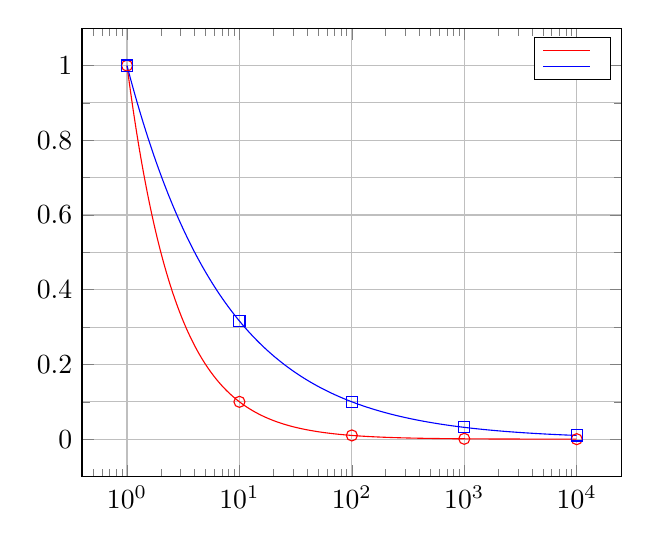
\begin{tikzpicture}
        \begin{axis}[xmajorgrids=true, ymajorgrids=true, xmode=log, yminorgrids=true, minor tick num = 1]
            \addplot[only marks, mark=o, color=red, forget plot] coordinates{(1, 1) (10, 0.1) (100, 0.01) (1000, 0.001) (10000, 0.00001)};
            \addplot[domain=1:10000, samples=1000, color=red]{1/x};
            \addplot[only marks, mark=square, color=blue, forget plot] coordinates{(1, 1) (10, 0.316) (100, 0.1) (1000, 0.032) (10000, 0.01)};
            \addplot[domain=1:10000, samples=1000, color=blue]{1/sqrt(x)};

            \addlegendentry{$\lint$}
            \addlegendentry{$\sqrtt$}
        \end{axis}
    \end{tikzpicture}
    \caption[Accumulating step function]{Comparison of decrease in value depending on time steps of two used step functions. These functions are used to compute the incremental average as described in \refsec{new:bandititeration:avg}}
    \label{new:bandititeration:steps}
\end{figure}

As can be seen from the figure \reffig{new:bandititeration:steps}, the $\sqrtt$ step function decreases slower than $\lint$ and thus can potentially lead to a faster convergence, because it will consider more recent values with higher weights than the older ones.
Please note, that the $x$ axis of the plot is displayed in the logarithmic scale.
However, we can no longer speak of the aggregation as of an arithmetic average.
These two step functions will be later compared on the bandit algorithms.

\subsection{Observable bandits}\label{new:bandititeration:obs}
When an observable variant of any stochastic multi-armed bandit algorithm is used in the \textit{bandit iteration} algorithm \refalg{new:bandititeration:alg}, the \textbf{receive} function looks a bit different.
These bandits need to receive both action $a_i$ selected by the owner and action $a_{-i}$ selected by the opponent together with the gained reward.
A more detailed description of observable bandit alternatives is located in section \refsec{new:bandit:obs}.

\section{B-HSVI}\label{new:bhsvi}
In \refsec{standard:osposg:hsvi}, a POMDP heuristic search value iteration modified for OS-POSGs \refsec{bg:osposg} was presented.
Even though this algorithm scales better in comparison to the exact method, it still uses linear programs as a method for solving stage games, which can lead to poor scalability.
With the use of multi-armed bandits presented in this and previous chapters \refchap{bandit}, we introduce an alternative method to solve the stages and find the equilibrial strategies.

\subsection{The algorithm}\label{new:bhsvi:alg}
From the original algorithm in \refsec{standard:osposg:hsvi:alg} the modified B-HSVI algorithm differs only in finding the equilibrial strategies of $[H\lb](b_t)$, resp. $[H\ub](b_t)$.
Thus, the only change in \refalg{standard:osposg:hsvi:alg:alg} is on the lines $7$, resp. $8$.

In \refalg{new:bhsvi:alg:alg:lb} is shown the extraction of a stage strategy profile from the lower bound $(\pi_1^{\text{LB}},\pi_2^{\text{LB}})$.
\begin{algorithm}
    \caption{Extract equilibrial strategies from $[H\lb](b_t)$}
    \label{new:bhsvi:alg:alg:lb}
    \begin{algorithmic}[1]
        \Require OS-POSG $G$, $\lb$, $\Gamma$, $b_t$
        \Ensure stage strategies $\pi_1^{\text{LB}}$, $\pi_2^{\text{LB}}$
        \State $\alpha \leftarrow$ select from $\Gamma$
        \State $B_1, B_2 \leftarrow$ bandit algorithms belonging to $\alpha$
        \State $a_1, a_2, \pi_1, \pi_2 \leftarrow$ retrieve current actions and strategies from $B_1$, $B_2$
        \State $\text{val}_{a_1}, \text{val}_{a_2}(s) \leftarrow$ compute bandit feedback $\forall s \in S$
        \State $B_1, B_2 \leftarrow a_1, \text{val}_{a_2}$ update state of the bandits
        \State $\Gamma \leftarrow \Gamma \cup \{\text{construct new } \alpha^{\prime} \text{ from } (\pi_1, \pi_2) \text{ in }b_t\}$
        \State $B_1^{\prime}, B_2^{\prime} \leftarrow$ copy bandits $B_1, B_2$ belonging to the new $\alpha^{\prime}$
        \State\Return $\pi_1, \pi_2$
    \end{algorithmic}
\end{algorithm}
The algorithm for the upper bound is analogous except for a few minor differences.
Instead of an $\alpha$-vector, a point $(b, y)$ is selected from $\Upsilon$ and then new point $(b^{\prime}, y^{\prime})$ is created and inserted to $\Upsilon$.

In each call of solving the stage game, i.e. lines $7, 8$ in the original algorithm, the procedure \refalg{new:bhsvi:alg:alg:lb} is performed.
First, an $\alpha$-vector, or a point $(b, y)$ is selected from its respective set.
In the case of the set $\Gamma$, the selection is partly randomized.
The elements of $\Gamma$ are sorted in decreasing order by their value in the current belief point $b_t$.
With probability $\epsilon = 0.1$ a random $\alpha$-vector from the first $10$ elements of the ordered $\Gamma$ is selected, with probability $(1 - \epsilon)$ the single best $\alpha$-vector.
This randomization prevents the algorithm from choosing a single $\alpha$-vector every time and creating new compositions which provide no improvement in value.
The point $(b, y)$ is selected by the belief point $b$.

Then we retrieve the bandit algorithms which belong to this selected $\alpha$-vector, whose strategy is meant to be refined.
Player 1 owns only a single bandit, while the player 2 has one bandit algorithm for each state $s \in S$.
From the bandits, the current actions are selected as well as the strategies played so far by these bandits.
Note, that while the bandit for the player 1 returns a single action $a_1$ and a single stage strategy $\pi_1$, the bandits of the player 2 are conditioned by the state $s$ and thus they provide mappings $a_1 : S \to A_1$ and $a_2 : S \to \Delta(A_2)$, which can conveniently be represented by vectors of length $|S|$.
The returned strategies correspond to relative frequencies of selections made by the bandit so far including this round, i.e. average play.

With these things prepared, the bandit feedback for the lower bound update is computed according to the following formula
\begin{equation}
    \text{val}_{a_2}(s) = R(s, a_1, a_2(s)) + \gamma \sum_{(o, \news) \in O \times S}T(o, \news \mid s, a_1, a_2(s)) \cdot \alpha^{a_1, o}(\news) \quad \forall s \in S,
\end{equation}
where $a_1, a_2$ are fixed by the selection from the bandits and $\alpha^{a_1, o}(\news)$ is a convex combination of the $\alpha$-vectors for the current pair $(a_1, o)$ evaluated in the simplex vertex $\news \in S$.
The upper bound formula is again analogous except that instead the $\alpha^{a_1, o}(\news)$, the lower convex hull of the points is computed and then evaluated in $\news$.
The value $\text{val}$ is then computed as
\begin{equation}
    \text{val}_{a_1} = \sum_{s \in S} b_t(s) \cdot \text{val}_{a_2}(s).
\end{equation}
This feedback is the passed to the bandits, however, the $\text{val}_{a_2}$ is multiplied by $-1$ to follow the maximization nature of the bandit algorithms.

Last, new $\alpha$-vector $\alpha^{\prime}$ or $(b^{\prime}, y^{\prime})$ is created based on the strategies returned by the bandits in this round.
These two operations are still conducted by a linear program.
The bandits $B_1$ and $B_2$ are then copied and assigned to this new object to allow independent continuation in case it is better than the former.

\subsubsection{Presolve}
For this procedure to work as described before, we need to alter the \textit{presolve} process in a similar fashion.
New bandits need to be initialized and assigned for every $\alpha$-vector and $(b, y)$ point.
These empty bandits then correspond to uniform strategies over $A_1$, resp. $A_2$.

\subsection{Performance}
This modification of the HSVI algorithm removes the need for solving a linear program to obtain the stage strategies in each step.
Instead, it uses strategies learned by the bandit algorithms corresponding to individual lower/upper bound elements.
However, the update of these strategies is changed only by a single action selection each round and thus can also change slowly in later phases of the learning.
In the next section, we compare different bandit algorithms and how they handle this slow changes.

The bandits are being copied because if their single selection was not in a good direction, in terms of creating $\alpha$-vector with lower value than the original, it would not compromise the original bandits and could be tried again.
This is also improved by the randomized element selection from $\Gamma$.

\section{Conclusion}
In this chapter, we summarized modifications of the bandit algorithms presented in chapter \refchap{bandit} to fit them more into game theory.
Next, we used these bandit algorithms to define an algorithm similar to value iteration called \textit{bandit iteration} to find solution of stochastic games without the need of computing linear programs.
Last, we incorporated the multi-armed bandits to the \textit{heuristic search value iteration} algorithm to create algorithm \textit{B-HSVI} solving OS-POSGs again to omit solving too many linear programs.

In the following chapter, we compare the specified bandit algorithms on SGs and OS-POSGs and how they influence convergence to the true values.
\end{document}
